% !TEX program = lualatex
% Generated by new_homework.sh — Math 113 Homework 5
\documentclass[11pt]{article}

\usepackage{fontspec}
\usepackage{microtype}
\usepackage{mathtools,amssymb,amsfonts,amsthm,bm}
\usepackage{enumitem}
\usepackage{booktabs,array,xcolor}
\usepackage{geometry,fancyhdr,setspace}
\usepackage{pdfpages}
\usepackage{graphicx}
\usepackage[hidelinks]{hyperref}
\usepackage[nameinlink,noabbrev]{cleveref}

% ---------- Page and paragraph rhythm (matches lecture/solutions templates) ----------
\geometry{margin=1in,headheight=15pt}
\setstretch{1.12}
\setlength{\parindent}{0pt}
\setlength{\parskip}{0.55em plus 0.12em minus 0.08em}
\setlength{\abovedisplayskip}{0.8em plus 0.2em minus 0.1em}
\setlength{\belowdisplayskip}{0.8em plus 0.2em minus 0.1em}
\allowdisplaybreaks[3]
\setlist{leftmargin=*,topsep=0.35em,itemsep=0.15em,parsep=0pt}

% ---------- Metadata ----------
\newcommand{\studentname}{Keshav Ramamurthy}
\newcommand{\coursename}{Math 113}
\newcommand{\courselongname}{Abstract Algebra}
\newcommand{\assignment}{Homework 5}
\newcommand{\term}{Fall 2026}

% ---------- Core notation (same as ~/.config/nvim/textemplate.tex) ----------
\newcommand{\N}{\mathbb{N}}
\newcommand{\Z}{\mathbb{Z}}
\newcommand{\Q}{\mathbb{Q}}
\newcommand{\R}{\mathbb{R}}
\newcommand{\C}{\mathbb{C}}
\newcommand{\F}{\mathbb{F}}
\newcommand{\K}{\mathbb{K}}
\newcommand{\E}{\mathbb{E}}
\newcommand{\Prob}{\mathbb{P}}
\newcommand{\1}{\mathbf{1}}
\newcommand{\eps}{\varepsilon}
\newcommand{\dd}{\,\mathrm{d}}
\newcommand{\abs}[1]{\left\lvert#1\right\rvert}
\newcommand{\norm}[1]{\left\lVert#1\right\rVert}
\newcommand{\ip}[2]{\left\langle#1,#2\right\rangle}
\newcommand{\set}[1]{\left\{#1\right\}}
\newcommand{\ceil}[1]{\left\lceil#1\right\rceil}
\newcommand{\floor}[1]{\left\lfloor#1\right\rfloor}
\newcommand{\given}{\,\middle\vert\,}
\newcommand{\indep}{\perp\!\!\!\perp}
\newcommand{\wh}[1]{\widehat{#1}}
\newcommand{\deriv}[2]{\frac{\mathrm{d}#1}{\mathrm{d}#2}}
\newcommand{\pderiv}[2]{\frac{\partial#1}{\partial#2}}
\newcommand{\lto}{\longrightarrow}
\newcommand{\st}{\text{ such that }}
\DeclareMathOperator{\Aut}{Aut}
\DeclareMathOperator{\End}{End}
\DeclareMathOperator{\Gal}{Gal}
\DeclareMathOperator{\Hom}{Hom}
\DeclareMathOperator{\Ker}{ker}
\DeclareMathOperator{\im}{im}
\DeclareMathOperator{\rank}{rank}
\DeclareMathOperator{\nullity}{nullity}
\DeclareMathOperator{\Span}{span}
\DeclareMathOperator{\tr}{tr}
\DeclareMathOperator{\diag}{diag}
\DeclareMathOperator{\spec}{spec}
\DeclareMathOperator{\ord}{ord}
\DeclareMathOperator{\supp}{supp}
\DeclareMathOperator{\diam}{diam}
\DeclareMathOperator{\Var}{Var}
\DeclareMathOperator{\Cov}{Cov}
\DeclareMathOperator*{\argmin}{arg\,min}
\DeclareMathOperator*{\argmax}{arg\,max}

% ---------- Statement environments ----------
\newtheorem{problem}{Problem}
\newtheorem{theorem}{Theorem}
\newtheorem{lemma}{Lemma}
\newtheorem{proposition}{Proposition}
\newtheorem{corollary}{Corollary}
\theoremstyle{definition}
\newtheorem{definition}{Definition}
\newtheorem{example}{Example}
\newtheorem{remark}{Remark}

% ---------- Solution machinery (matches solutions.tex / textemplate.tex) ----------
\newenvironment{solution}{\begin{proof}[Solution]}{\end{proof}}
\newenvironment{answer}{\begin{proof}[Answer]}{\end{proof}}
\renewcommand{\qedsymbol}{\(\square\)}
\newcommand{\exercise}[1]{%
  \par\goodbreak\medskip\noindent\textbf{Exercise #1}\par\nopagebreak\smallskip\nopagebreak}
\newcommand{\exref}[1]{\textsf{\textbf{Exercise~#1}}}
\newenvironment{claim}{\par\smallskip\noindent\textit{Claim.}\ }{\par\smallskip}
\newenvironment{idea}{\par\smallskip\noindent\textit{Idea.}\ }{\par\smallskip}
\newenvironment{proofsketch}{\par\smallskip\noindent\textit{Proof sketch.}\ }{\par\smallskip}

% ---------- Header ----------
\pagestyle{fancy}
\fancyhf{}
\fancyhead[L]{\coursename}
\fancyhead[C]{\assignment\ — my solutions}
\fancyhead[R]{\studentname}
\fancyfoot[C]{\thepage}

\begin{document}

% ---------- Title ----------
\begin{center}
  {\Large\sffamily\bfseries \coursename\ -- \courselongname}\par\vspace{3pt}
  {\sffamily \assignment\ — my solutions}\par\vspace{3pt}
  {\small\sffamily \term\quad\textbullet\quad \studentname}
\end{center}
\medskip
\hrule
\bigskip

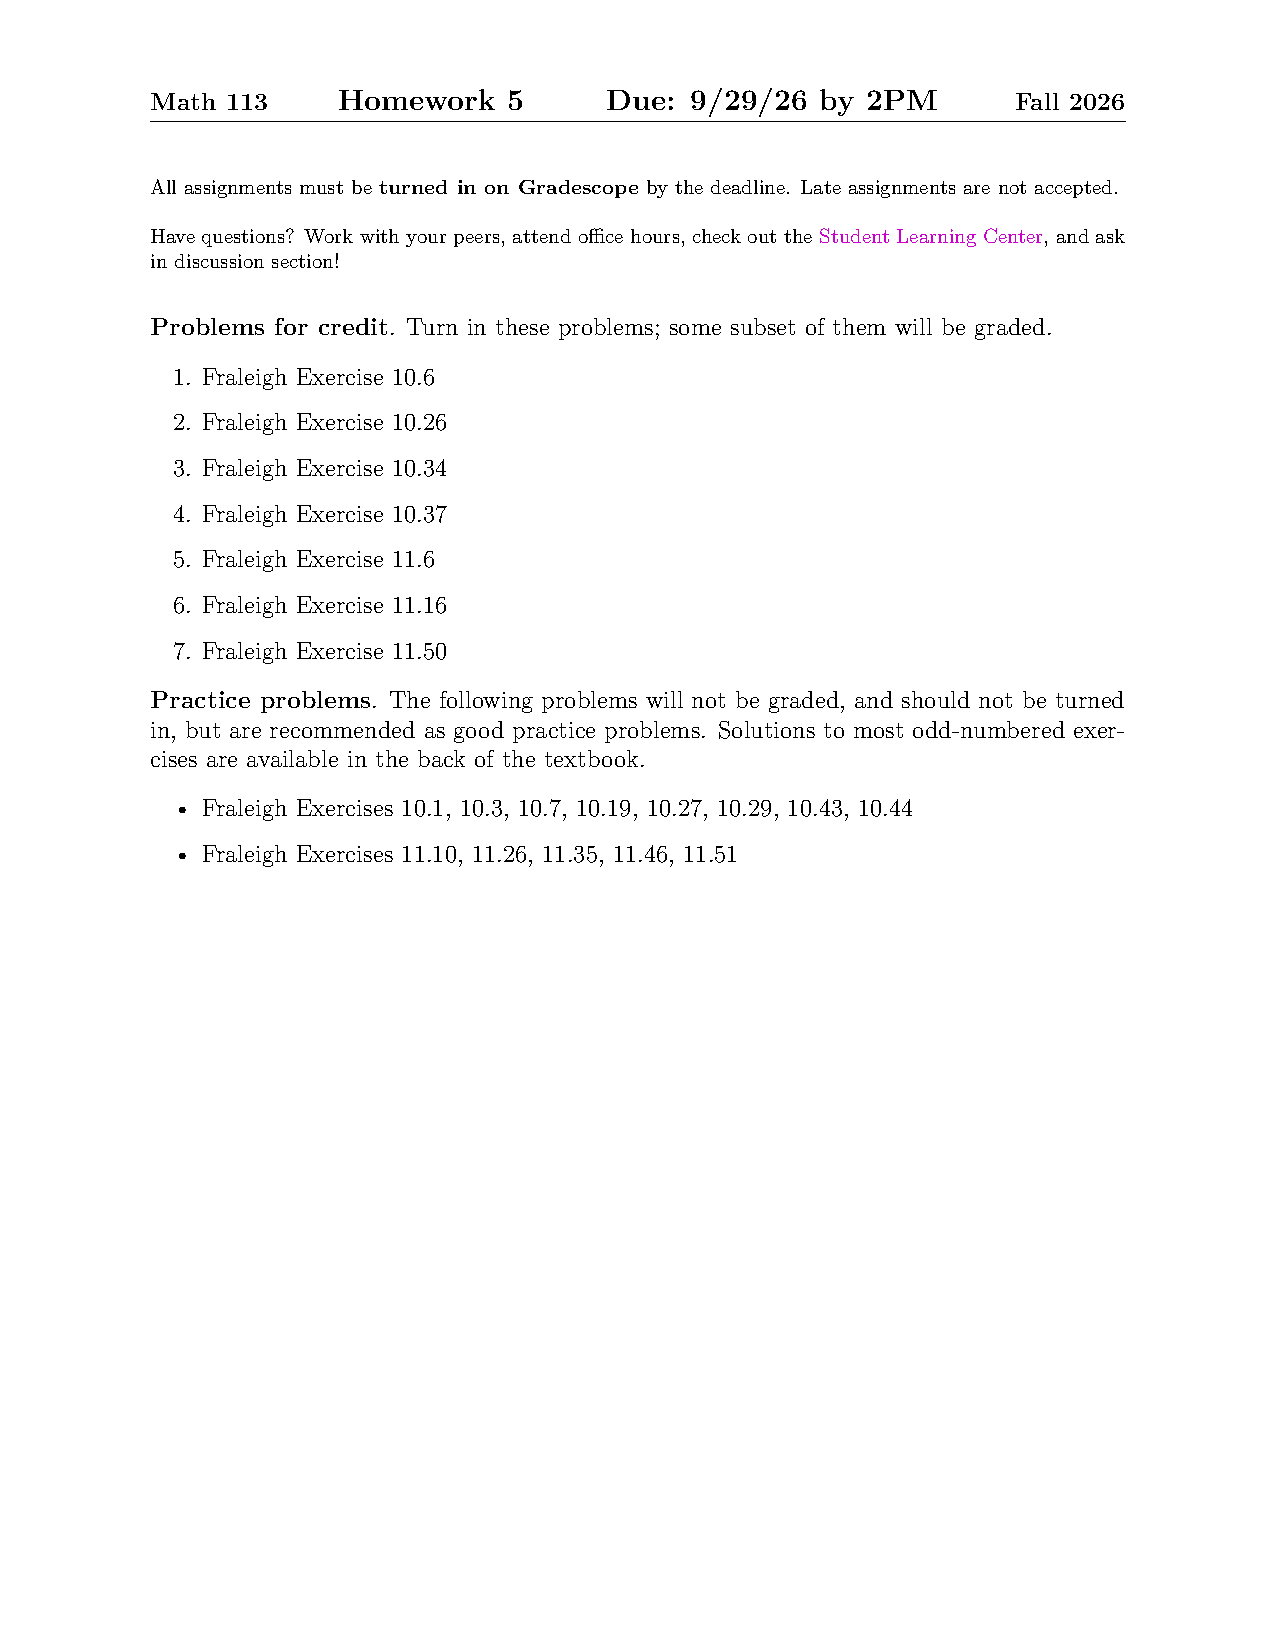
\includepdf[pages=-,pagecommand={\thispagestyle{empty}}]{hw5.pdf}
\clearpage

\section*{Solutions}
\subsubsection*{Problem 1 (Fraleigh Exercise 10.6)}
\begin{solution}
    % Reference for this exercise: Fraleigh Table 8.12 (multiplication table of
    % \(D_4\)) and Figure 8.13 (subgroup diagram of \(D_4\)). We need the left cosets
    % of the subgroup \(\{\rho_0, \mu_2\}\).
    \begin{center}
      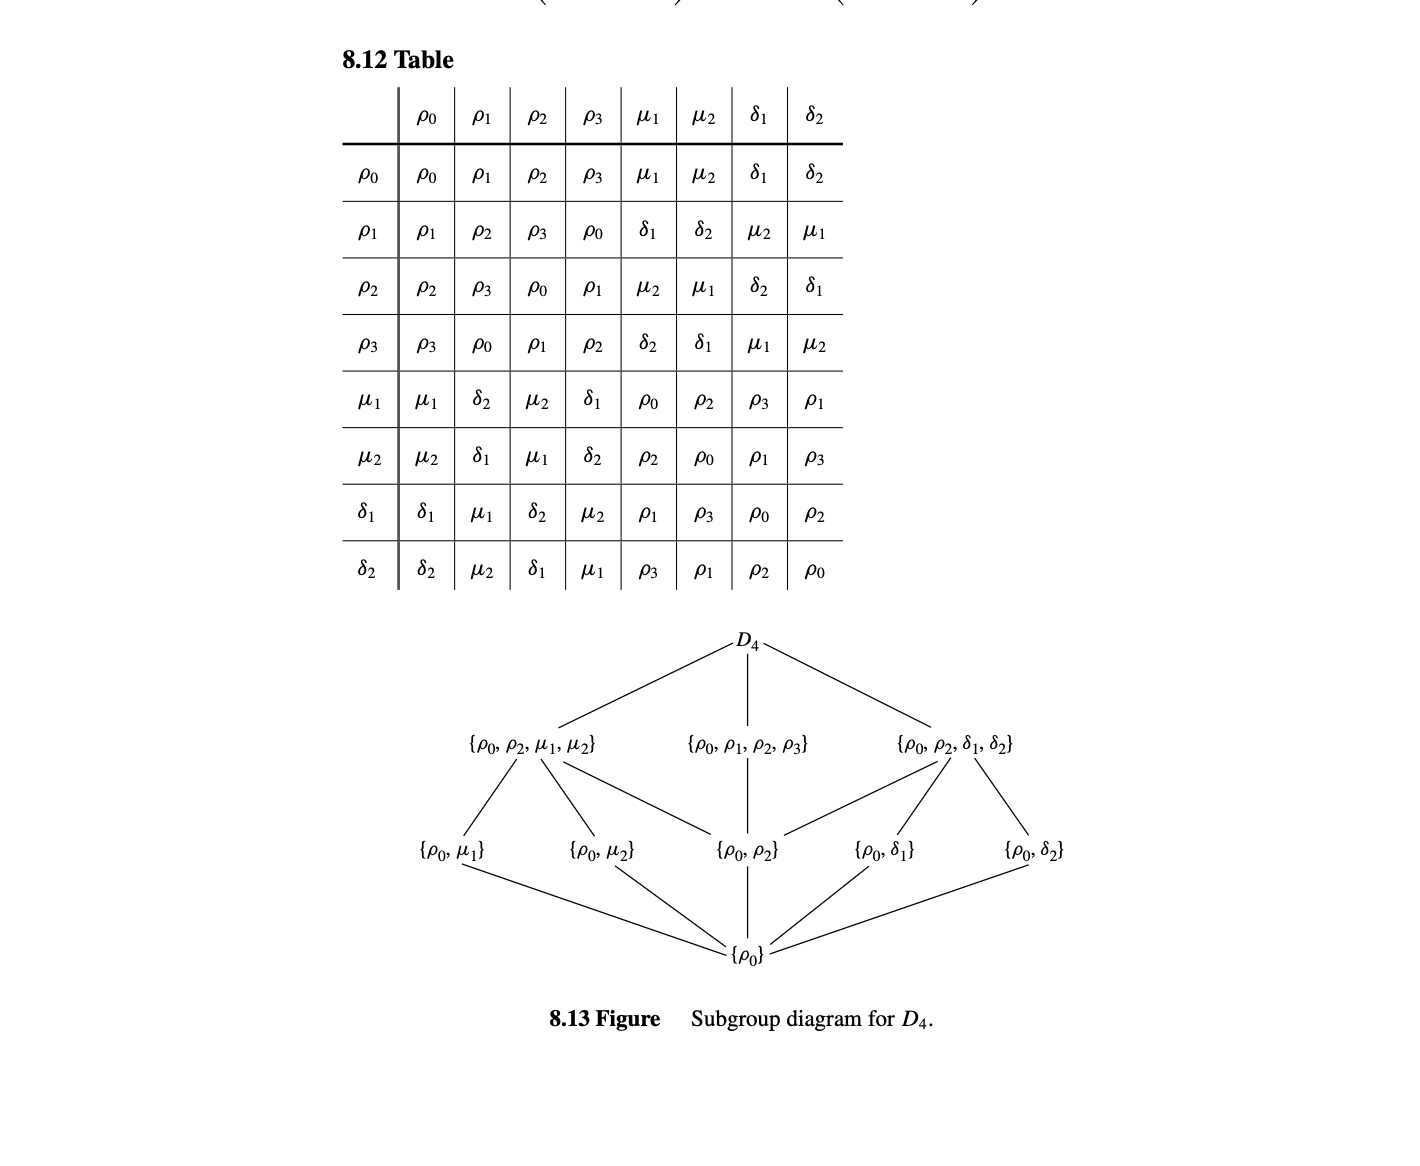
\includegraphics[width=0.92\linewidth]{hw05_problem1_d4_table812.png}
    \end{center}
    \(\rho_0\) is the identity and we are looking at the subgroup \(\{\rho_0, \mu_2\}\)
    \par The left cosets are of the form \(\{g\rho_0, g\mu_2\}\)
    So, going down the list we have 
    \[\rho_0(H) = \{\rho_0, \mu_2\}\]
    \[\rho_1(H)  = \{\rho_1 \rho_0, \rho_1\mu_2\}= \{\rho_1, \delta_2\}\]
    going off the table.
    Then 
    \[\rho_2(H) = \{\rho_2, \mu_1\}\]
    and 
    \[\rho_3(H) = \{\rho_3, \delta_1\}\]
    which is a partition of G.
% Write your proof, calculation, or argument here.
\end{solution}
\subsubsection*{Problem 2 (Fraleigh Exercise 10.26)}
\begin{solution}
    The equivalent relation is \(a \sim_R b \iff ab^{-1} \in H.\)
    \par We have to show reflexive, transitive, and symmetry.
    \par \textbf{Reflexive: } For \(a \in G\), \(aa^{-1} = e \in H \rightarrow aa^{-1} \in
    H.\)
    So we have that \(a \sim_R a.\)
\par    To show Symmetric, let's start from \(a\sim_R b\)
\par Then, there exists \(ab^{-1} \in H\) and from closure under inverses, we know that
\((ab^{-1})^{-1} \in H.\) \par Simplifying, this is  
\[(ab^{-1})^{-1} = (b^{-1})^{-1} a^{-1} = ba^{-1} \iff b \sim_R a\]
To show the transitive property, Let's start with \(a\sim_R b\) and \(b\sim_R c.\)
\par We have that \(ab^{-1} \in H\) and \(bc^{-1} \in H\) and since multiplication is closed,
we have \[(ab^{-1} )(bc^{-1}) = a(b^{-1}b)c^{-1} = ac^{-1} \iff a\sim_R c\]
% Write your proof, calculation, or argument here.
\end{solution}
\subsubsection*{Problem 3 (Fraleigh Exercise 10.34)}
\begin{solution}
    Given a group of order \(pq\) for prime p and q, we want to show that every proper
    subgroup of cyclic.
    \(|G| = pq\) so by lagrange   \(|H| \mid |G| \rightarrow |H| \in \{1, p, q\}\)
    \par \noindent\textit{Claim.} Every group with prime order is cyclic.
    \begin{proof}
        Consider an element \(h\in H, h\ne e.\)
        \par  By lagrange, the order of the subgroup \(\langle h \rangle\) must divide
    \(|H|= p\) so it is either 1 or \(|H|= p.\) 
    \par The \(\langle h\rangle = 1\) case would be \(\langle e\rangle
    \), but since \(h \ne e\), we have that  \(|H| = p\) and \(
    \langle h\rangle = H \) and H is cyclic.
    \end{proof}
    Also, if the subgroup of the group with order \(pq\) had size 1, it would be generated
    again by \(\langle e\rangle\) and thus be cyclic.
\par     Thus every proper subgroup must be cyclic.
% Write your proof, calculation, or argument here.
\end{solution}
\subsubsection*{Problem 4 (Fraleigh Exercise 10.37)}
\begin{solution}
    Consider an arbitrary group \(G\) with no proper non trivial subgroups.
    \par Take \(g \in G, g\ne e\) and let's examine \(\langle g\rangle \).
    \par Since there are no proper non trivial
    subgroups, we know that \(\langle g \rangle = G\) and G is cyclic.
 \par   If \(G\) was an infinite cyclic group, notice that \(\langle g^2\rangle = \{\cdots,
    g^{-4}, g^{-2}, e, g^{2}, g^{4}, \cdots \}\) is a proper non trivial subgroup, and
    elements like \(g^{2k+1}\) are not in this subgroup.
    \par  Thus this is a contradiction and \(G\) must be finite.
     \par If we suppose for sake of contradiction that \(|G|\) is composite, and is equal
     to \(|G| = pq, p \ne 1, q\ne 1\) for some values \(p\) and \(q\), we see for example that \(\langle
     g^{p}\rangle\) is a proper non trivial subgroup (and its order is \(\frac{n}{p} = q < |G|\))
     \par Thus we have a contradiction and \(G\) must be a cyclic group of prime order.
% Write your proof, calculation, or argument here.
\end{solution}
\subsubsection*{Problem 5 (Fraleigh Exercise 11.6)}
\begin{solution}
    Doing them separately, for the order of \(3\) in \(\mathbb{Z}_4\), it would be
    \(\frac{4}{\gcd(3, 4)} = 4\) 
    \par For \(10\) in \(\mathbb{Z}_{12}\), it would be \(\frac{12}{\gcd(10,12)}=6\)
    \par Lastly, for \(9\) in \(\mathbb{Z}_{15}\) it would be \(\frac{15}{\gcd(9,15)} = 5.\)
    Its a direct product, Taking the least common multiple of these we get 
    \[\text{lcm}(4, 6, 5) = 60\]
% Write your proof, calculation, or argument here.
\end{solution}
\subsubsection*{Problem 6 (Fraleigh Exercise 11.16)}
\begin{solution}
    We claim that \(\mathbb{Z}_2 \times \mathbb{Z}_{12}\)  and \(\mathbb{Z}_4 \times
    \mathbb{Z}_6\) are isomorphic.
    Since \(12 = 4 \cdot 3\) and \(3\) and \(4\) are relatively prime, \(\mathbb{Z}_{12} \cong
    \mathbb{Z}_3 \times \mathbb{Z}_4\) 
    Thus, \[\mathbb{Z}_2\times\mathbb{Z}_{12} \cong \mathbb{Z}_2\times
    \mathbb{Z}_3\times\mathbb{Z}_4\]
    Similarly using the fact that \(6 = 2\cdot 3\) and \(2\) and \(3\) relatively prime, we
    have that:
    \[\mathbb{Z}_4 \times \mathbb{Z}_6 \cong \mathbb{Z}_4 \times \mathbb{Z}_3\times
    \mathbb{Z}_2\]
    Since changing the orders preserve the isomorphism, we have that 
 \[\mathbb{Z}_4 \times \mathbb{Z}_6 \cong \mathbb{Z}_4 \times \mathbb{Z}_3\times
 \mathbb{Z}_2\cong \mathbb{Z}_2\mathbb{Z}_3\mathbb{Z}_4\]

    \[\mathbb{Z}_2 \times \mathbb{Z}_{12} \cong \mathbb{Z}_4\times\mathbb{Z}_6 \cong
\mathbb{Z}_2\times\mathbb{Z}_3\times\mathbb{Z}_4\]
as desired.
% Write your proof, calculation, or argument here.
    %
\end{solution}
\subsubsection*{Problem 7 (Fraleigh Exercise 11.50)}
\begin{solution}
   We have that \(G = H \times K\) and notice an element \((h, k) \in G\) can be written as
   \[(h, k)  = (h, e_K)(e_H, k) \text{ and } (h, e_K) \in H\times\{e\}, (e_H, k) \in \{e\}
   \times K\]
   So every element in \(G\) can be written as \(hk\) for \(h \in H, k\in K\) and we've shown
   \((a)\).
   \par For \((b)\),  we wish to show \(hk = kh\) for \(h\in H,k  \in K\), so consider 
   arbitrary\((h, e_K)\in H\) and \((e_H, k) \in K\) , we have that \[hk = (h,e_K)(e_H,k) =
   (he_H, e_Kk) = (h,k)\] and \[kh = (e_H,k)(h,e_K) = (e_Hh,ke_K)=(h,k)\] and thus
   \(hk = kh\)
   so we've shown part (b).
   \par To show part c which is $H \cap K = \{e\}$.
   \par To show this, consider an element $a \in H \cap K.$
   Then $$a = (h, e_K) = (e_H, k)\rightarrow h = e_H, e_K = k \text{ so } a = (e_H, e_K)
   = e_G$$
   and thus $H \cap K = \{e\}$
% Write your proof, calculation, or argument here.
\end{solution}

\end{document}
